% Exemplo de relatório técnico do IC

% Criado por P.J.de Rezende antes do Alvorecer da História.
% Modificado em 97-06-15 e 01-02-26 por J.Stolfi.
% modificado em 2003-06-07 21:12:18 por stolfi
% modificado em 2008-10-01 por cll
% modificado em 2010-03-16 17:56:58 por stolfi
% modificado em 2012-09-25 para ajustar o pacote UTF8. Contribuicao de Rogerio Cardoso
% \def\lastedit{2015-03-18 00:52:20 by bit}

\nonstopmode % PARA RODAR LATEX EM BATCH MODE
\documentclass[11pt,twoside]{article}

\usepackage{techrep-ic}

%%% SE USAR INGLÊS, TROQUE AS ATIVAÇÕES DOS DOIS COMANDOS A SEGUIR:
\usepackage[brazil]{babel}

\usepackage{makeidx}
%%% SE USAR CODIFICAÇÃO LATIN1 OU UTF-8, ATIVE UM DOS DOIS COMANDOS A
%%% SEGUIR:
%%\usepackage[latin1]{inputenc}
\usepackage[utf8]{inputenc}

%%% Para obter o tamanho de texto recomendado:
\usepackage[margin=1in]{geometry}

%%% Para colocar imagens:
\usepackage{graphicx}
\graphicspath{ {./images/} }

\usepackage{float}

\makeindex

\begin{document}

%%% PÁGINA DE CAPA %%%%%%%%%%%%%%%%%%%%%%%%%%%%%%%%%%%%%%%%%%%%%%%
%
% Número do relatório
\TRNumber{01} % Dois dígitos

% DATA DE PUBLICAÇÃO (PARA A CAPA)
%
\TRYear{18} % Dois dígitos
\TRMonth{6} % Numérico, 01-12

% LISTA DE AUTORES PARA CAPA (sem afiliações).
\TRAuthor{Ana Clara Zoppi Serpa - RA 165880
\and Bruno de Marco Apolonio - RA 195036
\and Gabriel Oliveira dos Santos - RA 197460
\and Lucas Costa de Oliveira - RA 182410
\and Vítor Mosso Dario - RA 207024}

% TÍTULO PARA A CAPA (use \\ para forçar quebras de linha).
\TRTitle{Grupo Caramelo: Sistema de gerenciamento de academia}

\TRMakeCover

%%%%%%%%%%%%%%%%%%%%%%%%%%%%%%%%%%%%%%%%%%%%%%%%%%%%%%%%%%%%%%%%%%%%%%
% O que segue é apenas uma sugestão - sinta-se à vontade para
% usar seu formato predileto, desde que as margens tenham pelo
% menos 25mm nos quatro lados, e o tamanho do fonte seja pelo menos
% 11pt. Certifique-se também de que o título e lista de autores
% estão reproduzidos na íntegra na página 1, a primeira depois da
% página de capa.
%%%%%%%%%%%%%%%%%%%%%%%%%%%%%%%%%%%%%%%%%%%%%%%%%%%%%%%%%%%%%%%%%%%%%%

%%%%%%%%%%%%%%%%%%%%%%%%%%%%%%%%%%%%%%%%%%%%%%%%%%%%%%%%%%%%%%%%%%%%%%
% Nomes de autores ABREVIADOS e titulo ABREVIADO,
% para cabeçalhos em cada página.
%

%%%%%%%%%%%%%%%%%%%%%%%%%%%%%%%%%%%%%%%%%%%%%%%%%%%%%%%%%%%%%%%%%%%%%%
% TÍTULO e NOMES DOS AUTORES, completos, para a página 1.
% Use "\\" para quebrar linhas, "\and" para separar autores.
%
\title{Caramelo: Sistema de gerenciamento de academia}

\author{
Ana Clara Zoppi Serpa
\and
Bruno de Marco Apolonio
\and
Gabriel Oliveira dos Santos
\and
Lucas Costa de Oliveira
\and
Vítor Mosso Dario
}

\date{}

\maketitle

%%%%%%%%%%%%%%%%%%%%%%%%%%%%%%%%%%%%%%%%%%%%%%%%%%%%%%%%%%%%%%%%%%%%%%

\begin{abstract}
Quisque accumsan ipsum id tortor laoreet feugiat. In accumsan id risus quis rutrum. Aliquam risus nunc, lacinia ac tincidunt at, accumsan ut purus. Morbi vestibulum et lacus at interdum. Cras pellentesque consectetur sapien, ac lobortis leo aliquam at. In consectetur nibh at bibendum laoreet. Aenean molestie lorem id mattis mattis. Integer rhoncus sem dictum, mattis massa vitae, pretium justo. Curabitur euismod dolor non neque semper tincidunt.

In congue consectetur risus eu pharetra. Vestibulum at lacus auctor, cursus leo et, placerat nibh. Suspendisse vitae enim justo. Praesent feugiat dolor accumsan dui euismod blandit. Maecenas interdum velit dolor, in laoreet urna feugiat finibus. Ut cursus eros id velit laoreet, at fringilla nibh ullamcorper. Donec aliquet elit nisi, quis pellentesque nibh molestie quis. Praesent volutpat hendrerit augue id molestie. Nullam orci ex, auctor non tristique vitae, dignissim at mauris. Fusce tempor eleifend aliquet. Class aptent taciti sociosqu ad litora torquent per conubia nostra, per inceptos himenaeos. Proin mollis ligula id laoreet dignissim.
\end{abstract}

\clearpage
\tableofcontents

\clearpage

\section{Etapa 0: Proposta de Software}
Nessa etapa, decidimos qual seria o tema do nosso projeto e quais suas funcionalidades.
Optamos por implementar um sistema de gerenciamento de academias com cadastro de clientes, atividades
e instrutores e a associação destes, por exemplo: o cliente Gabriel faz pilates
de segunda e quarta, das 16h às 17h, e o instrutor responsável pelas aulas de pilates desse horário é o Lucas.

Escrevemos um documento descrevendo as funcionalidades que prevíamos para o sistema e entregamos para o professor.
Como elas já foram descritas no documento, aqui são mencionadas mais brevemente:

\begin{itemize}
  \item Cadastro dos clientes que frequentam a academia
  \item Alteração dos dados de um cliente já cadastrado
  \item Desativar um cliente
  \item Cadastro de atividades que a academia oferece
  \item Alteração dos dados da atividade, por exemplo, preço
  \item Remoção de uma atividade
  \item Associar/desassociar horários às atividades oferecidas
  \item Associar/desassociar clientes aos horários e atividades
  \item Cadastrar instrutores que trabalham na academia
  \item Alterar dados de um instrutor cadastrado
  \item Desativar um instrutor
  \item Consultar qual atividade possui mais clientes
  \item Consultar qual atividade possui menos clientes
  \item Consultar qual atividade tem o maior preço
  \item Consultar qual atividade tem o menor preço
\end{itemize}

Em vez de remover clientes e instrutores, optamos por desativá-los. Tivemos essa ideia pensando no seguinte cenário: um cliente
decide deixar de frequentar a academia, mas, após algum tempo, retorna. Seria prático se já tivéssemos os dados dele e bastasse
reativá-lo. O mesmo ocorre com instrutores que parem de trabalhar na academia, mas depois retornem. Ou, por exemplo, a academia
talvez tenha interesse em tentar contactar um instrutor para contratá-lo novamente, ou um cliente antigo para perguntar se ele
deseja retornar.

\section{Etapa 1: Classes do sistema}
Nessa etapa, pensamos sobre as classes e relacionamentos entre elas e construímos um diagrama UML. O professor indicou correções,
as quais realizamos em outras etapas. O diagrama a seguir está parcialmente correto e o apresentamos apenas para facilitar a
compreensão das ideias.

\begin{figure}[H]
\centering
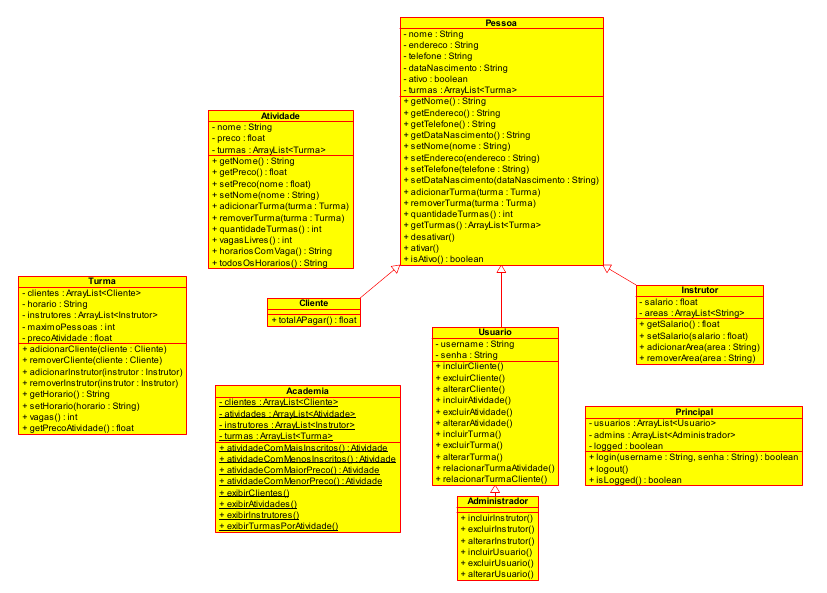
\includegraphics[width=.75\textwidth]{uml0}
\caption{Diagrama UML para a Release 0}
\end{figure}

Decidimos que o relacionamento entre cliente, horário, atividade e instrutor seria feito por meio de uma nova classe, a classe
Turma, da seguinte forma:

\begin{itemize}
  \item Uma atividade possui n turmas.
  \item Uma turma possui n clientes, n instrutores e um horário que representaremos com o tipo String.
  \item Um cliente possui n turmas, afinal, ele pode realizar várias atividades diferentes.
  \item Um instrutor possui n turmas porque ele pode dar aulas em várias turmas diferentes.
\end{itemize}

Percebemos que clientes e instrutores possuiriam nome, endereço, telefone, data de nascimento, lista de turmas e a indicação
de que estão ou não ativos no sistema como atributos em comum. Portanto, decidimos criar a classe Pessoa com esses atributos, getters e
setters
e fazer com que clientes
e instrutores fossem suas subclasses.

O cliente possui, além dos métodos e atributos da classe Pessoa, o método que calcula quanto ele precisa pagar pelas atividades
realizadas.

Como uma atividade possui n turmas, mas as turmas possuem apenas clientes, instrutores e horário, ou seja, a turma não sabe
qual é a sua atividade, decidimos, por questões de facilidade, guardar o preço da atividade na classe Turma também. Dessa forma,
para calcular quanto o cliente precisa pagar, basta iterar por sua lista de turmas e acumular os preços.

O instrutor possui, além dos métodos e atributos da classe Pessoa, um atributo salário e uma lista de áreas
(que representamos com uma lista de Strings) nas quais atua.

A classe Academia seria nossa base de dados, guardando em listas todos os clientes, instrutores, atividades e turmas do sistema
e possuindo métodos para exibí-los.

Decidimos também implementar uma etapa de login no sistema e separar os usuários entre usuários comuns e usuários administradores.
Um usuário comum poderia incluir/alterar/remover/desativar clientes, atividades e turmas, enquanto um usuário administrador
poderia fazê-lo também para instrutores e usuários. Portanto, administrador é uma subclasse de usuário.

Usuários possuem username e senha. Nessa etapa do projeto, pensamos em fazer com que Usuário fosse subclasse de Pessoa, para
guardarmos também seus dados (nome, endereço, telefone, data de nascimento).

\section{Etapa 2: Release 0}
Para essa Release, iniciamos a implementação seguindo o diagrama UML construído na Etapa 1. Criamos as classes em Java, seus métodos
e implementamos alguns deles, deixando outros vazios para serem implementados posteriormente.

\section{Etapa 3: Release 1}
Para essa Release, implementamos os métodos que, na anterior, estavam vazios. Realizamos algumas mudanças ao perceber alternativas
e necessidades não previstas.

\begin{itemize}
  \item
\end{itemize}

% Não teve como colocar o diagrama porque ele é muito grande e, se reduz, fica impossível de ler.

Atualizamos o diagrama UML para que refletisse essas mudanças, acrescentando algumas correções mencionadas
pelo professor (cardinalidades, associações, agregações etc).

Também fizemos alguns protótipos de interface gráfica (telas) para o software.

O professor sugeriu que implementássemos métodos de busca, por exemplo, buscar clientes por nome/endereço/telefone e
aumentássemos a complexidade do sistema acrescentando mais conceitos de Programação Orientada a Objetos, como herança e
polimorfismo. Isso foi feito nas releases seguintes.

\section{Etapa 4: Release 2}
- colocamos conceitos de POO e buscas
- mais interface gráfica
\section{Release final}
- colocamos o login que tínhamos tirado
- mais interface gráfica
\end{document}
